\section{Results}\label{sec:results}
In this section, we use CMC to estimate the posterior parameter distribution for three biological systems.
% of interest targeting synthetic parametric densities. That is,
In all but one of examples, we assume that the first step of CMC (``SnapshotEstimator'' within Algorithm \ref{alg:cmc}) has already been undertaken and we are faced with inferring a parameter distribution which, when mapped to outputs, recapitulates the target density. To accompany the text, we provide the Julia notebook used to generate the results. %, which we hope will be of use to others wanting to apply CMC to estimate cell population heterogeneity.
A table of priors used for each example is provided in Table \ref{tab:priors}.


\subsection{Growth factor model}
We first consider the ``growth factor model'' introduced by \cite{dixit2018maximum}, which concerns the dynamics of inactive ligand-free cell surface receptors $R$ and active ligand-bound cell surface receptors $P$, modulated by an exogenous ligand $L$. The governing dynamics are determined by the following system,
%
\begin{align}\label{eq:growth_factor}
\frac{dR}{dt} &= R_T k_{deg} + k_1 L R(t) + k_{-1} P(t) - k_{deg} R(t)\\
\label{eq:growth_factor1}
\frac{dP}{dt} &= k_1 L R(t) - k_{-1} P(t) - k^*_{deg} P(t),
\end{align}
with initial conditions
\begin{equation*}
R(0) = ??? \qquad P(0) = ???
\end{equation*}
%
where $\boldsymbol{\theta}=(R_T, k_1, k_{-1}, k_{deg}, k^*_{deg})$ are parameters to be determined. In this example, we use measurements of the active ligand-bound receptors $P$ to estimate cellular heterogeneity in processes. We denote the solution of eq. (\ref{eq:growth_factor1}) as $P(t; \boldsymbol{\theta}, L)$ and seek to determine the parameter distribution consistent with an output distribution,
%
\begin{equation}\label{eq:MM_outputDistribution}
\boldsymbol{q} =
\begin{pmatrix}
q_1\\
q_2\\
\end{pmatrix}
=
\begin{pmatrix}
P(10; \boldsymbol{\theta}, 2)\\
P(10; \boldsymbol{\theta}, 10)\\
\end{pmatrix} \sim  \mathcal{N}
\begin{bmatrix}
\begin{pmatrix}
2\times 10^4\\
3\times 10^4\\
\end{pmatrix}, \;\;
\begin{pmatrix}
1\times 10^5 & 0\\
0 & 1\times 10^5\\
\end{pmatrix}
\end{bmatrix}.
\end{equation}
%

\subsubsection{Uniform prior}
To start, we specify a uniform prior for each of the five parameters, with bounds given in Table \ref{tab:priors}. To estimate the posterior parameter distribution, we use CMC, with adaptive covariance MCMC \cite{johnstone2016uncertainty} for the second step.

In Figure \ref{fig:growth_factor_outputs}A, we show the sampled outputs (blue points) versus the contours of the target distribution (black solid closed curves), illustrating a good correspondence between the sampled and target densities. Above and to the right of the main panel, we also display the marginal target densities (solid black lines) versus kernel density estimator reconstructions of the output marginals from the CMC samples (dashed blue lines), which again highlights the fidelity of the CMC sampled density to the target.

\begin{figure}[H]
	\centerline{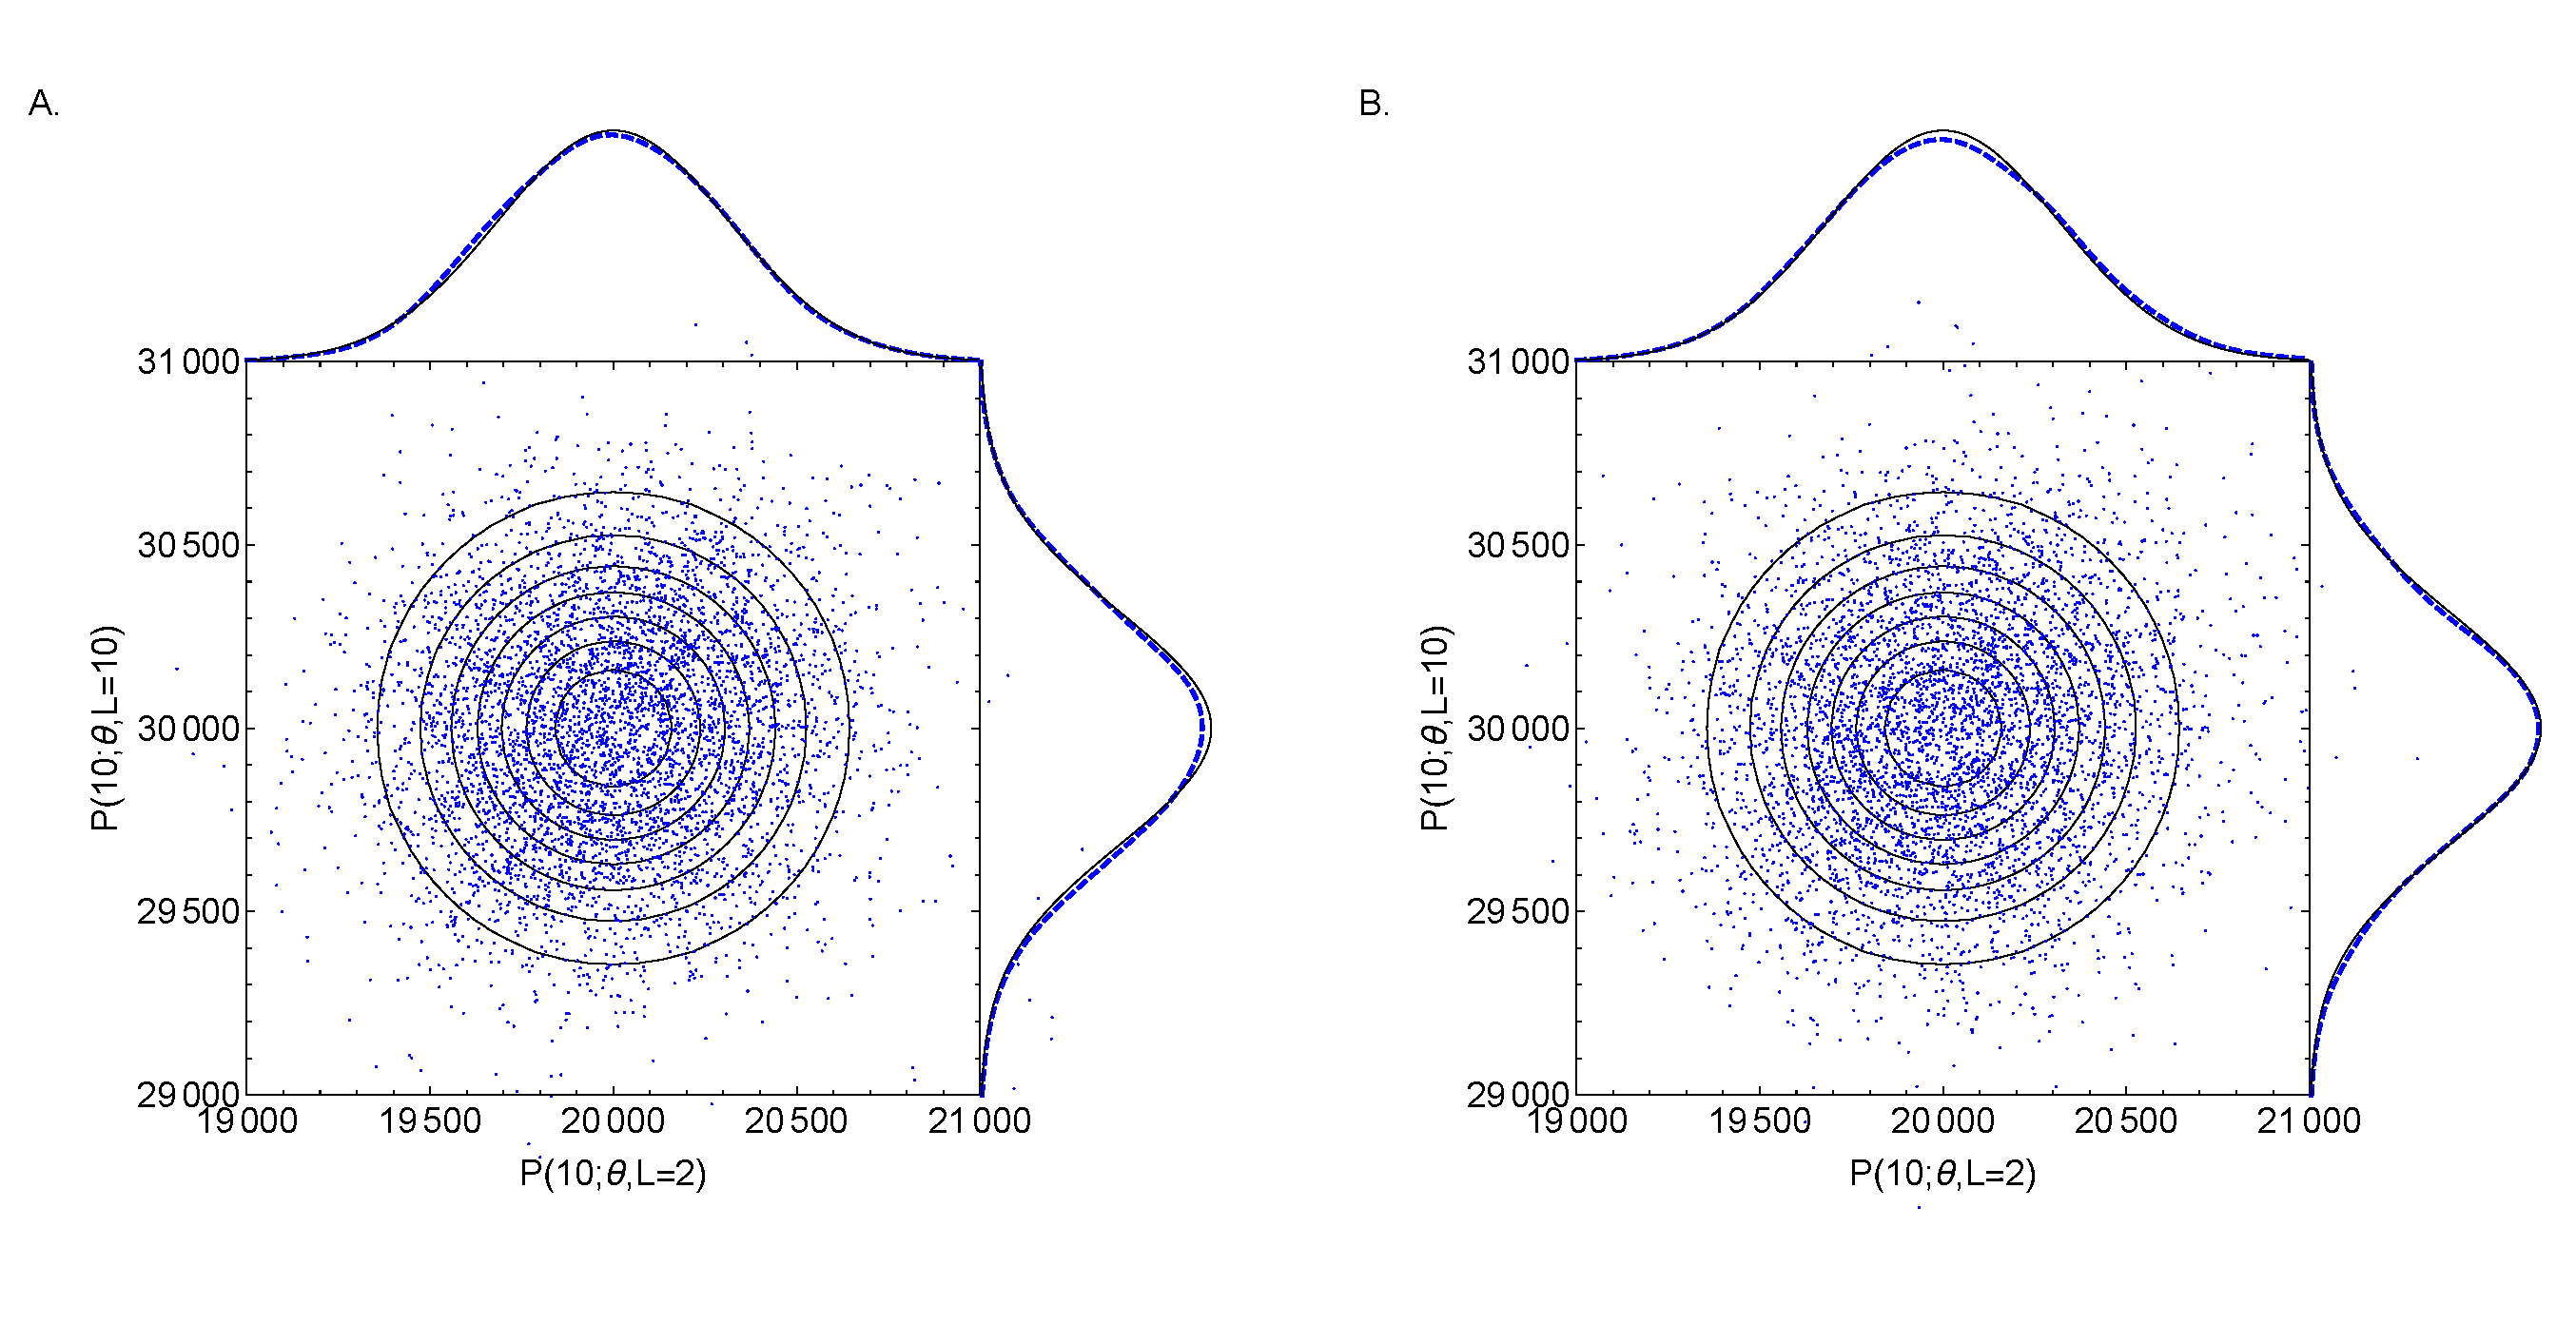
\includegraphics[width=\textwidth]{../figures/growth_factor_outputs.pdf}}
	\caption{\textbf{The target joint output distribution (solid contour lines) and target marginal distributions (solid lines; above and to side of figure) versus outputs sampled by CMC (blue points and dashed lines) for (A) uniform and (B) normal parameter priors.} In CMC, 100,000 independent samples were used in the ``ContourVolumeEstimator'' step and 10,000 MCMC samples across each of 4 Markov chains were used in the second step, with the first half of the chains discarded as ``warm-up'' \cite{lambert2018Student}. For the reconstructed marginal densities in the plots, we use Mathematica's ``SmoothKernelDistribution'' function specifying bandwidths of 100 with Gaussian kernels \cite{mathematica}.}
	\label{fig:growth_factor_outputs}
\end{figure}

\centerline{\tt SJT: What are the contour levels that are plotted?}

In Figure \ref{fig:growth_factor_inputs}A, we plot the joint posterior parameter distribution for $k_1$, the rate of ligand binding to inactive receptors, and $k_{-1}$, which dictates the rate of the reverse reaction, where the ligands unbind. The output measurements we used to fit the model correspond to levels of the bound ligands, which can be generated whenever the ratio of $k_1$ to $k_{-1}$ is approximately given by the corresponding steady state ratio. Because of this, the distribution representing cell process heterogeneity contains linear positive correlations between these parameters. In Figure \ref{fig:growth_factor_inputs}B, we show the posterior parameter distribution for $k_{deg}$, the rate of degradation of ligand-free cell surface receptors and $R_T$, which dictates the rate of introduction of ligand-free cell surface receptors, which shows a concentrated region of posterior probability mass. Why is it that we are better able to resolve $(k_{deg},R_T)$ compared to $(k_1,k_{-1})$ from our measurements? To answer this, it is useful to calculate the sensitivity of $P(t; \boldsymbol{\theta}, L)$ to changes in each of the parameters. To account for the differing magnitudes of each parameter, we calculate elasticities, the proportional changes in measured output for a proportional change in parameter values, using the forward sensitivities method described in \cite{DGCT2018}, which are shown in Figure \ref{fig:dixit_elasticities}. When the exogenous ligand is set $L=2$, these indicate the active ligand-bound receptor concentration is most elastic to changes in $R_T$ and $k_{deg}$, meaning that their range is more restricted by the output measurement than for $k_1$ and $k_{-1}$, which have elasticities at $t=10$ closer to 0. In Table \ref{tab:growth_factor_results}, we show the posterior quantiles for the estimated parameters and, in the last column, indicate the ratio of the 25\%-75\% posterior interval widths to the uniform prior range for each parameter. These were strongly negatively correlated with the magnitude of the elasticities for each parameter ($\rho=0.95$, $t=-5.22$, $df=3$, $p=0.01$ Pearson's product-moment correlation), indicating the utility of sensitivity analyses for optimal experimental design. We would suggest however that CMC can also be used for this purpose, using synthetic data in place of real measurements.


\begin{figure}[H]
	\centerline{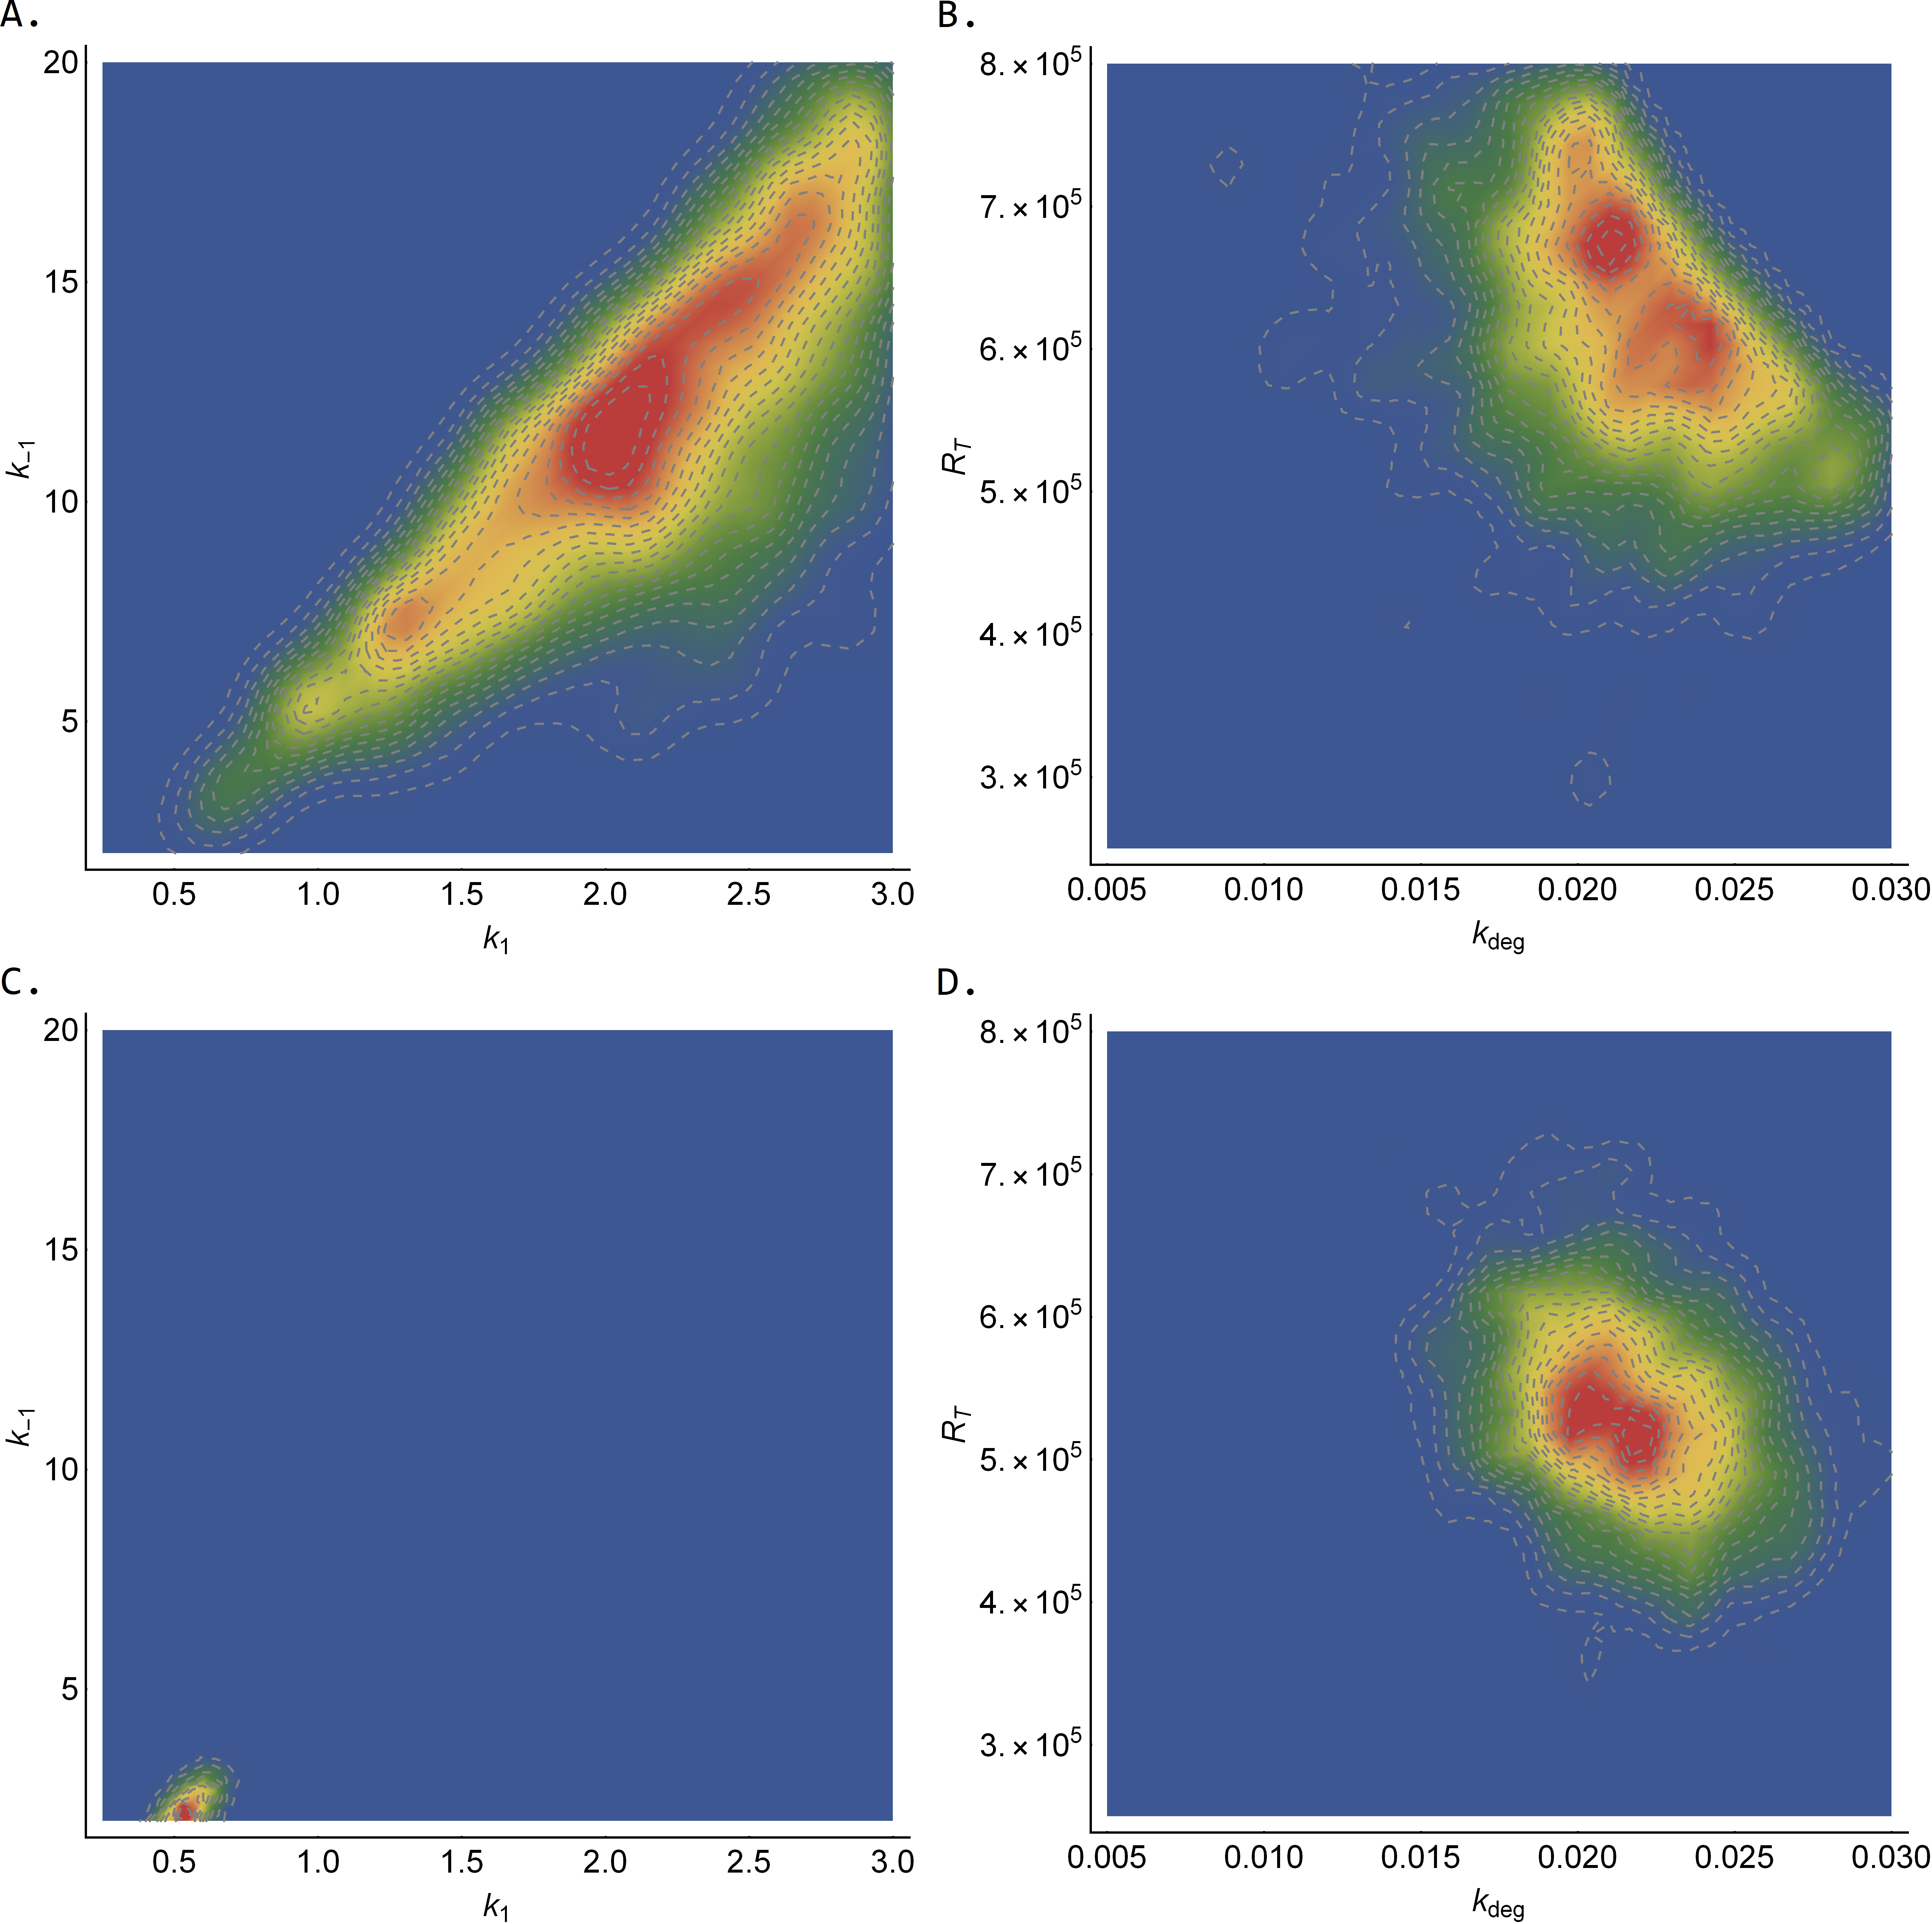
\includegraphics[width=\textwidth]{../figures/growth_factor_inputs.png}}
	\caption{\textbf{The joint distributions of $(k_1,k_{-1})$ (left-column) and $(k_{deg},R_T)$ for the growth factor model using uniform priors (top row) and normal priors (bottom row).} See Figure \ref{fig:growth_factor_outputs} caption for CMC details and Table \ref{tab:priors} for the priors used.}
	\label{fig:growth_factor_inputs}
\end{figure}

\begin{figure}[H]
	\centerline{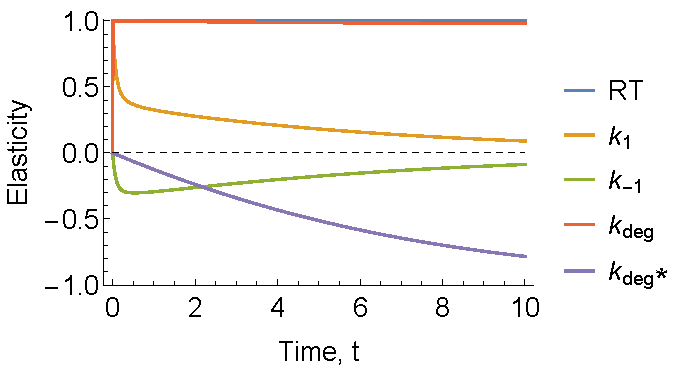
\includegraphics[width=0.7\textwidth]{../figures/dixit_elasticities.pdf}}
	\caption{\textbf{The elasticities of the measured concentration of active ligand-bound receptors $P$ versus time when $L=2$.} When calculating the elasticities of each parameter, the other parameters were set to their posterior medians given in Table \ref{tab:growth_factor_results}.}
	\label{fig:dixit_elasticities}
\end{figure}

\subsubsection{Specified prior}
For an unidentified model, there is typically a multitude of possible probability distributions over parameters which map to the same target output distribution. To reduce the space of posterior parameter distributions to one, it is therefore necessary to specify a prior parameter distribution. It is also preferable to allow priors to influence estimates in studies of cellular heterogeneity, since this allows incorporation of pre-existing biological knowledge with compensatory reductions in estimator variance. CMC accommodates different prior choices, with both the ``ContourVolumeEstimation'' step and the acceptance ratio in the ``MCMC'' step (Algorithm \ref{alg:cmc}) being affected in such a way that posterior parameter distribution maps to the same output target. We now use CMC to estimate the posterior parameter distribution when changing from uniform priors to more concentrated normal priors (prior hyperparameters shown in Table \ref{tab:priors}). As desired, the target output distribution appears invariant (Figure \ref{fig:growth_factor_outputs}B) although with substantial changes in the posterior parameter distributions (Figure \ref{fig:growth_factor_inputs}C\&D). In particular, the posterior distributions obtained from shifting to the normal prior are more concentrated in parameter space compared to the uniform case (rightmost column of Table \ref{tab:growth_factor_results}). The differences in posterior distribution resultant from changes to priors are likely to be more marked the less definitive a guide the data provides on the underlying process and, hence, can be used to stabilise the resultant inferences according to external knowledge about the system.

\begin{table}
%	\scriptsize
\begin{tabular}{c|ccccc|c}
\toprule
&&&&&&                                         Posterior \\
Parameter &  \multicolumn{5}{c}{Quantiles} &   25\%-75\% \\
          & 2.5\% & 25\% & 50\% & 75\% & 97.5\% & conc.\\
\toprule
\multicolumn{7}{c}{Uniform prior} \\
\toprule
$R_T$       &  441,006 & 548,275 & 606,439 & 677,055 & 772,484 & 23\%\\
$k_1$       &  0.90 & 1.69 & 2.17 & 2.56 & 2.95 & 32\%\\
$k_{-1}$    & 4.35 & 8.35 & 11.23 & 14.23 & 18.71 & 33\%\\
$k_{deg}$   & 0.013 & 0.019 & 0.021 & 0.024 & 0.029 & 20\%\\
$k^*_{deg}$ & 0.20 & 0.34 & 0.40 & 0.44 & 0.49 & 27\%\\
\toprule
\multicolumn{7}{c}{Normal prior} \\
\toprule
$R_T$       & 408,396 & 487,372 & 529,558 & 577,970 & 678,632 & 16\%\\
$k_1$       & 0.39 & 0.49 & 0.54 & 0.60 & 0.70 & 4\%\\
$k_{-1}$    & 1.39 & 1.92 & 2.26 & 2.63 & 3.35 & 4\%\\
$k_{deg}$   & 0.016 & 0.020 & 0.022 & 0.024 & 0.027 & 16\%\\
$k^*_{deg}$ & 0.22 & 0.29 & 0.33 & 0.38 & 0.46 & 21\%\\
\end{tabular}
\caption{\textbf{Estimated quantiles from CMC samples for the growth factor model with uniform and normal priors.} The last column indicates the proportion of the uniform prior bounds occupied by the 25\%-75\% posterior interval in each case. The particular priors used in each case are given in Table \ref{tab:priors}.}
\label{tab:growth_factor_results}
\end{table}

\subsection{Michaelis-Menten kinetics}
In this section, we use CMC to invert output measurements from the Michaelis-Menten model of enzyme kinetics (see, for example, \cite{murray2007mathematical}); illustrating the capability of CMC to resolve population substructure from multimodality of the output distribution. The Michaelis-Menten model of enzyme kinetics describes the dynamics of concentrations of an enzyme ($E$), a substrate ($S$), an enzyme-substrate complex ($ES$), and a product ($P$). Specifically,
%
\begin{equation}\label{eq:michaelis_menten}
\begin{aligned}
\frac{dE}{dt} &= -k_f E(t)S(t) + k_r C(t) + k_{cat} C(t), \\
\frac{dS}{dt} &= -k_f E(t)S(t) + k_r C(t), \\
\frac{dC}{dt} &= \phantom{-}k_f E(t)S(t) - k_r C(t) - k_{cat} C(t), \\
\frac{dP}{dt} &= \phantom{-}k_{cat} C(t),
\end{aligned}
\end{equation}
%
with initial conditions,
\begin{equation}
E(0) = E_0, \; S(0)=S_0, \; C(0)=C_0, \; P(0)=P_0,
\end{equation}
%
where $k_f$ is the rate constant for the forward reaction $E+S \rightarrow C$, $k_r$ is the rate of the reverse reaction $C \rightarrow E+S$, and $k_{cat}$ is the catalytic rate at which the product is formed by the reaction $C \rightarrow E + P$.


\subsubsection{Bimodal output distribution}

When subpopulations of cells, each with distinct dynamics, are thought to exist, determining their characteristics - proportions of overall cell number, likely parameter values, and so on - is often of key interest \cite{hasenauer2011identification,loos2018hierarchical}. Before formal inference occurs, multi-modality of the output distribution may signal the existence of fragmented subpopulations of cells. Here we target the following bimodal bivariate normal distribution,
%
\begin{align}
\boldsymbol{q} = \begin{pmatrix} q_1 \\ q_2 \end{pmatrix}
 = \begin{pmatrix} E(2; \boldsymbol{\theta}) \\ S(1; \boldsymbol{\theta}) \end{pmatrix}
&  \sim
\boldsymbol{\Phi}(\boldsymbol{q}; \boldsymbol{\mu}_1,\Sigma_1, \boldsymbol{\mu}_2, \Sigma_2) \\
&= \frac{1}{2}\left(\mathcal{N}(\boldsymbol{q}; \boldsymbol{\mu}_1,\Sigma_1)
+ \mathcal{N}(\boldsymbol{q}; \boldsymbol{\mu}_2,\Sigma_2)\right),
\end{align}
%
%where $\boldsymbol{x} = \left(E(2; \boldsymbol{\theta}), S(1; \boldsymbol{\theta})\right)$ with each element corresponding to the solutions of eq. (\ref{eq:michaelis_menten}) for the enzyme and substrate at times $t=2$ and $t=1$, respectively, and
where $\boldsymbol{\theta}=(k_f,k_r,k_{cat})$. The parameters of the mixture normal output distribution we target are
\begin{equation*}
\begin{aligned}
&\boldsymbol{\mu}_1=[2.2, 1.6]', \; \Sigma_1 = \begin{pmatrix}0.018 & -0.013 \\ -0.013 & 0.010 \end{pmatrix}, \\
&\boldsymbol{\mu}_2=[2.8, 1.0]', \; \Sigma_2 = \begin{pmatrix}0.020 & -0.010 \\ -0.010 & 0.020 \end{pmatrix}.
\end{aligned}
\end{equation*}
In what follows, we specify uniform priors on each of the elements of $\boldsymbol{\theta}$ (see Table \ref{tab:priors}).


Using a modest number of samples in each step, CMC was able to recapitulate the output target distribution (Figure \ref{fig:mm_bimodal_inputs_outputs}A). Without specifying \textit{a priori} information on the subpopulations of cells, two distinct clusters of cells emerged from application of CMC (orange and blue points in Figure \ref{fig:mm_bimodal_inputs_outputs}B), each corresponding to distinct modes of the output distribution (corresponding coloured points in Figure \ref{fig:mm_bimodal_inputs_outputs}A). It is worth noting however that the issues inherent with MCMC sampling of multimodal distributions similarly apply here and so, whilst here adaptive MCMC \cite{johnstone2016uncertainty} sufficed to explore the posterior surface, it may be necessary to use MCMC methods known to be robust to such geometries (for example, population MCMC \cite{jasra2007population}).

\begin{figure}[H]
\centerline{\includegraphics[width=\textwidth]{../figures/mm_bimodal_inputs_outputs.pdf}}
\caption{\textbf{Michaelis-Menten model. (A) Bimodal target distribution $\boldsymbol{q}$ (solid contour lines) versus output samples (points). (B) Posterior parameter samples (points).} The solid and dashed lines above and to the side of panel A indicate the target and estimated marginal output distributions, respectively. The orange (blue) points in A were generated by the orange (blue) parameter samples in B. %See Figure \ref{fig:growth_factor_outputs} caption for CMC details.
Mathematica's ``SmoothKernelDistribution'' function \cite{mathematica} with Gaussian kernels was used to construct marginal densities with: (A) default bandwidths, and (B) bandwidths of 0.3 (horizontal axis) and 0.03 (vertical axis). Mathematica's ``ClusteringComponents'' function \cite{mathematica} was used to identify clusters %by applying to the pairs of parameter samples displayed
in B.}
\label{fig:mm_bimodal_inputs_outputs}
\end{figure}

\subsubsection{Four-dimensional output distribution}

Loos et al. (2018) consider a multidimensional output distribution, with correlations between system characteristics that evolve over time. Our approach allows arbitrary covariance structure between measurements, and to exemplify this, we now target a four-dimensional output distribution, with paired measurements of enzyme and substrate at $t=1$ and $t=2$,
%
\begin{equation}\label{eq:MM_4d_output}
\begin{aligned}
\boldsymbol{q} = \begin{pmatrix} q_1 \\ q_2 \\ q_3 \\ q_4 \end{pmatrix} &=
\begin{pmatrix}
E(1.0; \boldsymbol{\theta})\\
S(1.0; \boldsymbol{\theta})\\
E(2.0; \boldsymbol{\theta})\\
S(2.0; \boldsymbol{\theta})\\
\end{pmatrix}
\\
&\sim  \mathcal{N}
\begin{bmatrix}
\begin{pmatrix}
0.5\\
2.8\\
0.9\\
1.4\\
\end{pmatrix}, \;\;
\begin{pmatrix}
0.02 &  -0.05 &  0.04 & -0.05\\
-0.05 & 0.30  & -0.15 & 0.20\\
0.04 & -0.15  & 0.12  &  -0.17\\
-0.05 & 0.20 & -0.17 & 0.30
\end{pmatrix}
\end{bmatrix}.
\end{aligned}
\end{equation}
%
Since this system has four output measurements, and the Michaelis-Menten model has three rate parameters $(k_f,k_r,k_{cat})$, the system is over-identified and so CMC cannot be straightforwardly applied. Instead, we allow the four initial states $(E_0, S_0, ES_0, P_0)$ to be uncertain quantities, bringing the total number of parameters to 7, and ensuring that the system is in the unidentified regime where CMC applies. We set uniform priors on all parameters (see Table \ref{tab:priors}) and to check that the model and priors were consistent with the output distribution given by eq. (\ref{eq:MM_4d_output}), we plotted the output measurements used to estimate contour volumes (in the first step of the ``ContourVolumeEstimator'' method in Algorithm \ref{alg:cmc}) against the target (Figure \ref{fig:mm_4d_main}). Since the main support of the densities (black contours) lies within a region of output space reached by independent sampling of the priors (blue points), this indicated that the distribution given by eq. (\ref{eq:MM_4d_output}) could feasibly be generated from this model and priors, and we proceeded to estimation by CMC.

\begin{figure}[H]
\centerline{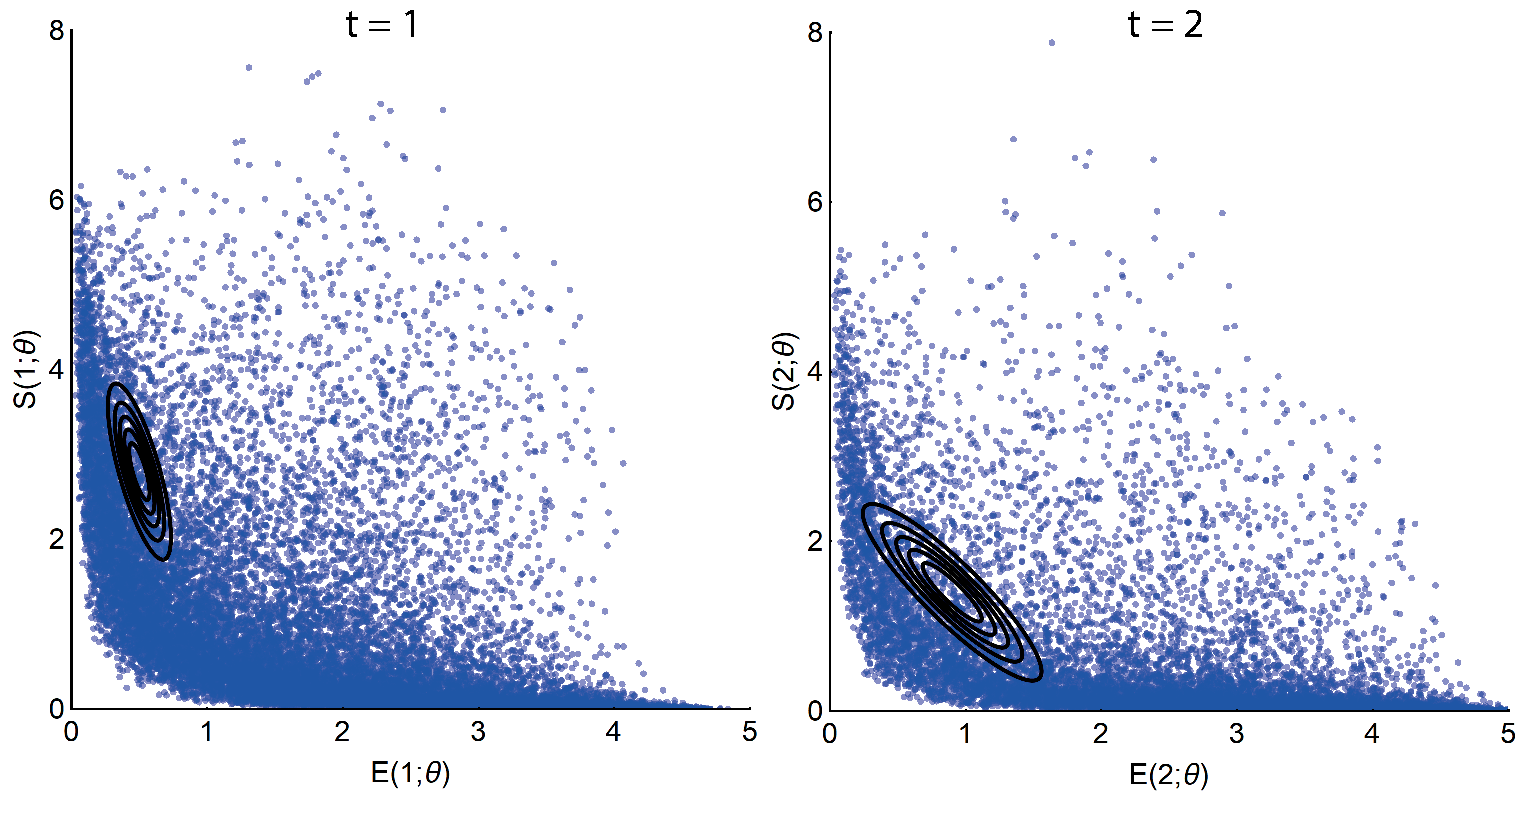
\includegraphics[width=\textwidth]{../figures/mm_4d_main.pdf}}
\caption{\textbf{Output functionals (blue points) $(q_1,q_2)$ (left panel) and $(q_3,q_4)$ (right panel) obtained by independently sampling the priors $p(\boldsymbol{q} | \boldsymbol(\Psi)$ of the 7 parameter Michaelis-Menten model versus the target distribution (black solid contours).} We show 20,000 output samples, where each set of four measurements was obtained from a single sample of the 7 parameters. The output target distribution shown by the contours corresponds to the marginal densities of each pair of enzyme-substrate measurements given by eq. (\ref{eq:MM_4d_output}).}
\label{fig:mm_4d_main}
\end{figure}
{\tt SJT: Ben please check my caption for Figure \ref{fig:mm_4d_outputs} is correct.}

Figure \ref{fig:mm_4d_outputs} plots the output samples of enzyme and substrate from the last step of CMC for $t=1$ (blue points) and $t=2$ (orange points) versus the contours (black lines) of the joint marginal distributions of eq. (\ref{eq:MM_4d_output}). The distribution of paired enzyme-substrate samples illustrates that the CMC output samples approximated the target density, itself representing dynamic evolution of the covariance between enzyme and substrate measurements. The target marginal distributions (solid lines) along with their approximations from kernel density estimation (dashed lines) are also shown above and beside the main panel of Figure \ref{fig:mm_4d_outputs}, and largely indicate correspondence.

\begin{figure}[H]
\centerline{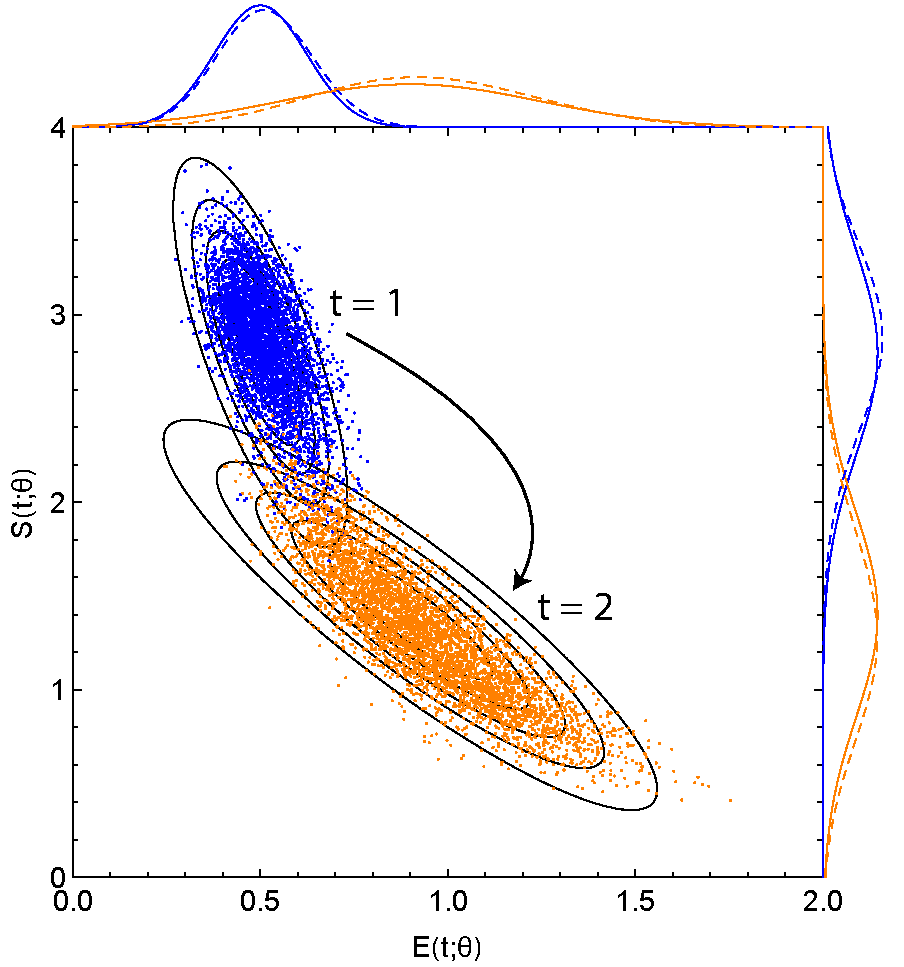
\includegraphics[width=0.65\textwidth]{../figures/mm_4d_outputs.pdf}}
\caption{\textbf{Posterior output samples from CMC (coloured points) versus the contour plots of the joint marginal distributions of eq. (\ref{eq:MM_4d_output}) (black solid lines).} Output functionals $(q_1,q_2)$ (blue) and $(q_3,q_4)$ (orange). Enzyme (horizontal axis) and substrate (vertical axis). The solid and dashed coloured lines outside of the panels indicate the true target marginals of eq. (\ref{eq:MM_4d_output}) and those estimated from CMC, respectively. %The line colours correspond with the point colours and indicate the marginals for $t=1$ (blue) and $t=2$ (orange).
200,000 independent samples were used in the ``ContourVolumeEstimator'' and 10,000 samples across each of 4 Markov chains were used in the MCMC step, with the first half of the chains discarded as ``warm-up'' \cite{lambert2018Student}. Mathematica's ``SmoothKernelDistribution'' function with Gaussian kernels \cite{mathematica} of bandwidths varying from 0.1 to 0.4 for the reconstructed marginal densities.}
\label{fig:mm_4d_outputs}
\end{figure}


\subsection{TNF signalling pathway}
We now illustrate how CMC can be applied to an ODE system of larger size, the tumour necrosis factor (TNF) signalling pathway model introduced in \cite{chaves2008bistable} and used by \cite{hasenauer2011identification} to illustrate a Bayesian approach to cell population variability estimation. The model incorporates known activating and inhibitory interactions between four key species within the TNF pathway: active caspase 8 ($x_1$) and active caspase 3 ($x_2$), a nuclear transcription factor ($x_3$) and its inhibitor ($x_4$),
%
\begin{equation}\label{eq:tnf}
\begin{aligned}
\frac{dx_1}{dt} &= -x_1(t) + \frac{1}{2}\left(\beta_4(x_3(t))\alpha_1(u(t)) + \alpha_3(x_2(t))\right)\\
\frac{dx_2}{dt} &= -x_2(t) + \alpha_2(x_1(t)) \beta_3(x_3(t))\\
\frac{dx_3}{dt} &= -x_3(t) + \beta_2(x_2(t)) \beta_5(x_4(t))\\
\frac{dx_4}{dt} &= -x_4(t) + \frac{1}{2}\left(\beta_1(u(t)) + \alpha_4(x_3(t))\right),
\end{aligned}
\end{equation}
%
with initial conditions
\begin{equation}
x_1(0)=0.0, \quad x_2(0)=0.0, \quad x_3(0)=0.29, \quad x_4(0)=0.625,
\end{equation}
which correspond to the steady state of the system when $x_2=0$. The functions $\alpha_i$ and $\beta_j$ represent activating and inhibitory interactions respectively,
%
\begin{equation}
\begin{aligned}
\alpha_i(z) &= \frac{z^2}{a_i^2 + z^2}, \quad i=1, \dots, 4,\\
\beta_j(z)  &= \frac{b_j^2}{b_j^2 + z^2}, \quad j = 1, \dots, 5,
\end{aligned}
\end{equation}
%
and the parameters $a_i$ for $i\in(1,2,3,4)$ and $b_j$ for $j\in(1,2,3,4,5)$ represent activation and inhibition thresholds. The function $u(t)$ represents a TNF stimulus which is given by a top hat function,
%
\begin{equation}
u(t)=\begin{cases}
1, & \text{if $t\in[0,2]$}.\\
0, & \text{otherwise}.
\end{cases}
\end{equation}
%
When there are fewer output measurements than parameters, models tend to be underdetermined meaning that many combinations of parameters can lead to the same combination of output values. A consequence of this unidentifiability is that we cannot perform ``full circle'' inference: that is, using a known parameter distribution to generate an output distribution does not result in that parameter distribution being recapitulated through inference. We illustrate this idea by generating an output distribution by varying a single parameter value between runs of the forward model corresponding to the solution of eq. (\ref{eq:tnf}) and performing inference on all nine system parameters, whilst collecting only two output measurements. Specifically, we vary $a_1\sim \mathcal{N}(0.6, 0.05)$, whilst holding the other parameters constant $$(a_2,a_3,a_4,b_1,b_2,b_3,b_4,b_5)=(0.2, 0.2, 0.5, 0.4, 0.7, 0.3, 0.5, 0.4)$$ and measure $q_1=x_1(2.0)$ and $q_2=x_2(1.0)$. By solving the forward model using Algorithm \ref{alg:simulate}, we obtain an output distribution that is well approximated by the bivariate normal distribution,
%
\begin{equation}\label{eq:tnf_circular_target}
\begin{aligned}
\boldsymbol{q} = \begin{pmatrix} q_1 \\ q_2 \end{pmatrix}
&=
\begin{pmatrix}
x_1(2.0)\\
x_2(1.0)\\
\end{pmatrix} \\
&\sim  \mathcal{N}
\begin{bmatrix}
\begin{pmatrix}
0.26\\
0.07\\
\end{pmatrix}, \;\;
\begin{pmatrix}
2.1\times 10^{-4} & 5.9\times 10^{-5}\\
5.9\times 10^{-5} & 1.8\times 10^{-5}\\
\end{pmatrix}
\end{bmatrix}.
\end{aligned}
\end{equation}
%
We now apply CMC to the target output distribution given by eq. (\ref{eq:tnf_circular_target}) to estimate a posterior distribution over all nine parameters of eq. (\ref{eq:tnf}). Apart than for a few cases, the priors for each parameter were chosen to \emph{exclude} the values that were used to generate the output distribution (see Table \ref{tab:priors}), to illustrate the non-equivalence between the recovered posterior distribution and the data generating process. In Figure \ref{fig:tnf_circular_versus}A, we plot the actual parameter values (horizontal axis) used in the true data generating process versus the inferred values (vertical axis). This illustrates that apart from $a_1$, where the estimated parameter values correspond well with the range of values used to generate the data, due to the choice of priors there is a disjunction between the actual and estimated values. Despite these differences, due to the model being underdetermined, it is nonetheless possible to use CMC to sample from an output distribution that well approximates the target (Figure \ref{fig:tnf_circular_versus}B).


\begin{figure}[H]
\centerline{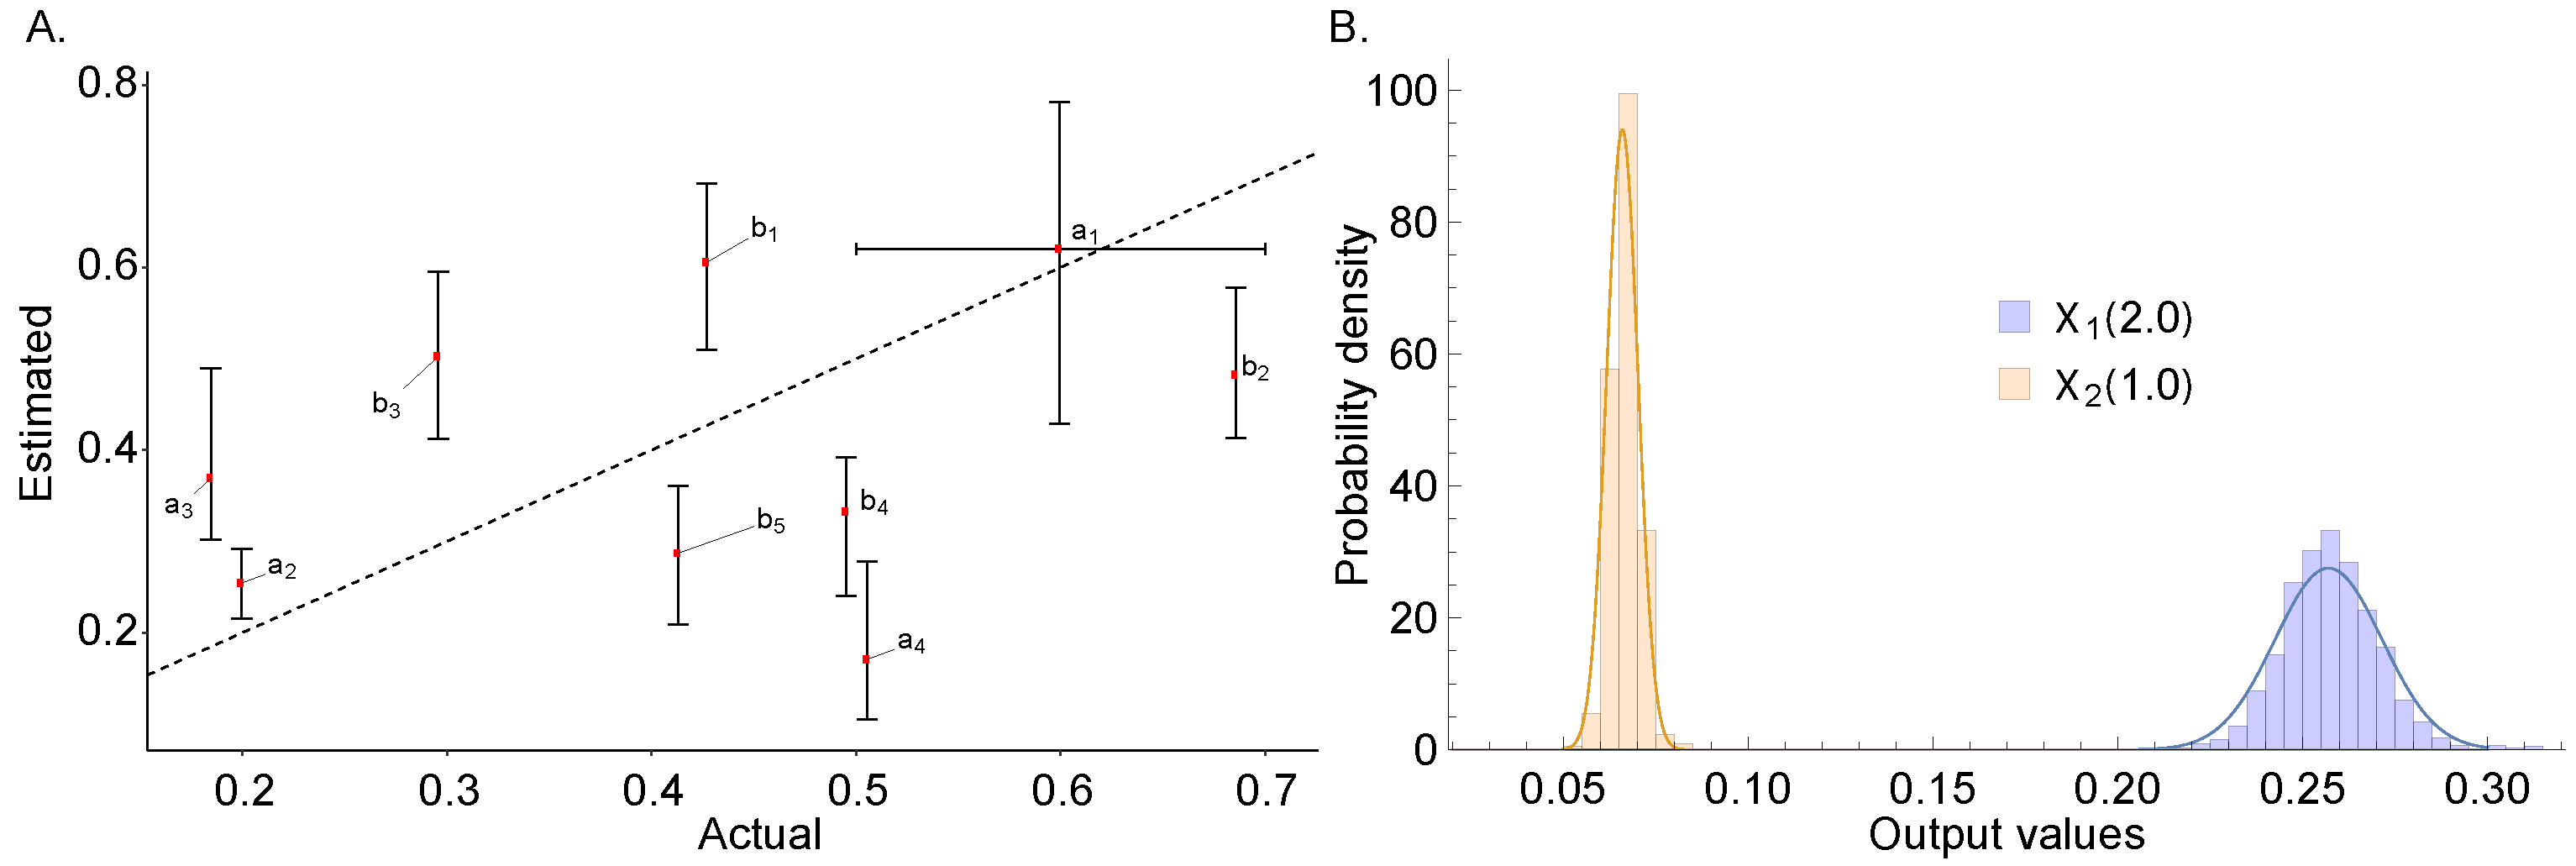
\includegraphics[width=1\textwidth]{../figures/tnf_circular_both.pdf}}
\caption{\textbf{(A) actual parameter values versus estimated quantiles for the output distribution for the TNF signalling pathway model with output distribution given and (B) the marginal output target (solid lines) given by eq. (\ref{eq:tnf_circular_target}) and sampled output distribution (histograms).} In A, in the vertical direction, the red points indicate the 50\% posterior quantiles and the upper and lower whiskers indicate the 97.5\% and 2.5\% quantiles, respectively; in the horizontal direction, with the exception of $a_1$, the red points indicate the parameter values used to generate the data; for $a_1$ the red point indicates the mean of the normal distribution used to generate the data and the whiskers indicate the 95\% quantiles of this distribution. In CMC, 10,000 independent samples were used in the ``ContourVolumeEstimator'' step and 5,000 MCMC samples across each of 4 Markov chains were used in the second step, with the first half of the chains discarded as ``warm-up'' \cite{lambert2018Student}.}
	\label{fig:tnf_circular_versus}
\end{figure}

Cell populations may be well described by subpopulations which each evolve along characteristic trajectories over time. We now apply CMC to investigate a bimodal output distribution for the TNF signalling pathway model similar to that investigated by \cite{hasenauer2011identification}. In particular, we aim to find a distribution over parameter values which, when used as inputs to the solution to the ODE system, results in the following output distribution,
%
\begin{equation}
\boldsymbol{q} = \begin{pmatrix} q_1 \\ q_2 \\ q_3 \end{pmatrix}
\end{equation}
where
\begin{equation}
\begin{aligned}
q_1 = \boldsymbol{x}_2(1.0) &\sim \mathcal{N}(0.06, 0.01)\\
q_2 = \boldsymbol{x}_2(2.0) &\sim\frac{1}{2}\left(\mathcal{N}(0.1, 0.01) + \mathcal{N}(0.14, 0.01)\right)\\
q_3 = \boldsymbol{x}_2(4.0) &\sim\frac{1}{2}\left(\mathcal{N}(0.1, 0.01) + \mathcal{N}(0.20, 0.01)\right),\\
\end{aligned}
\end{equation}
%
where the target distributions for $\boldsymbol{q}_2(2.0)$ and $\boldsymbol{q}_2(4.0)$ indicate mixtures of univariate normals, and the priors used are shown in Table \ref{tab:priors}. This target distribution, along with the unique trajectories obtained by applying the CMC algorithm for 5,000 MCMC steps, are shown in Figure \ref{fig:tnf_samples_vs_distribution}. This figure illustrates that given by bimodality of the output distribution, CMC estimates a corresponding subpopulation structure in the parameter distribution without \textit{a priori} specification of the number of clusters.

\begin{figure}[H]
	\centerline{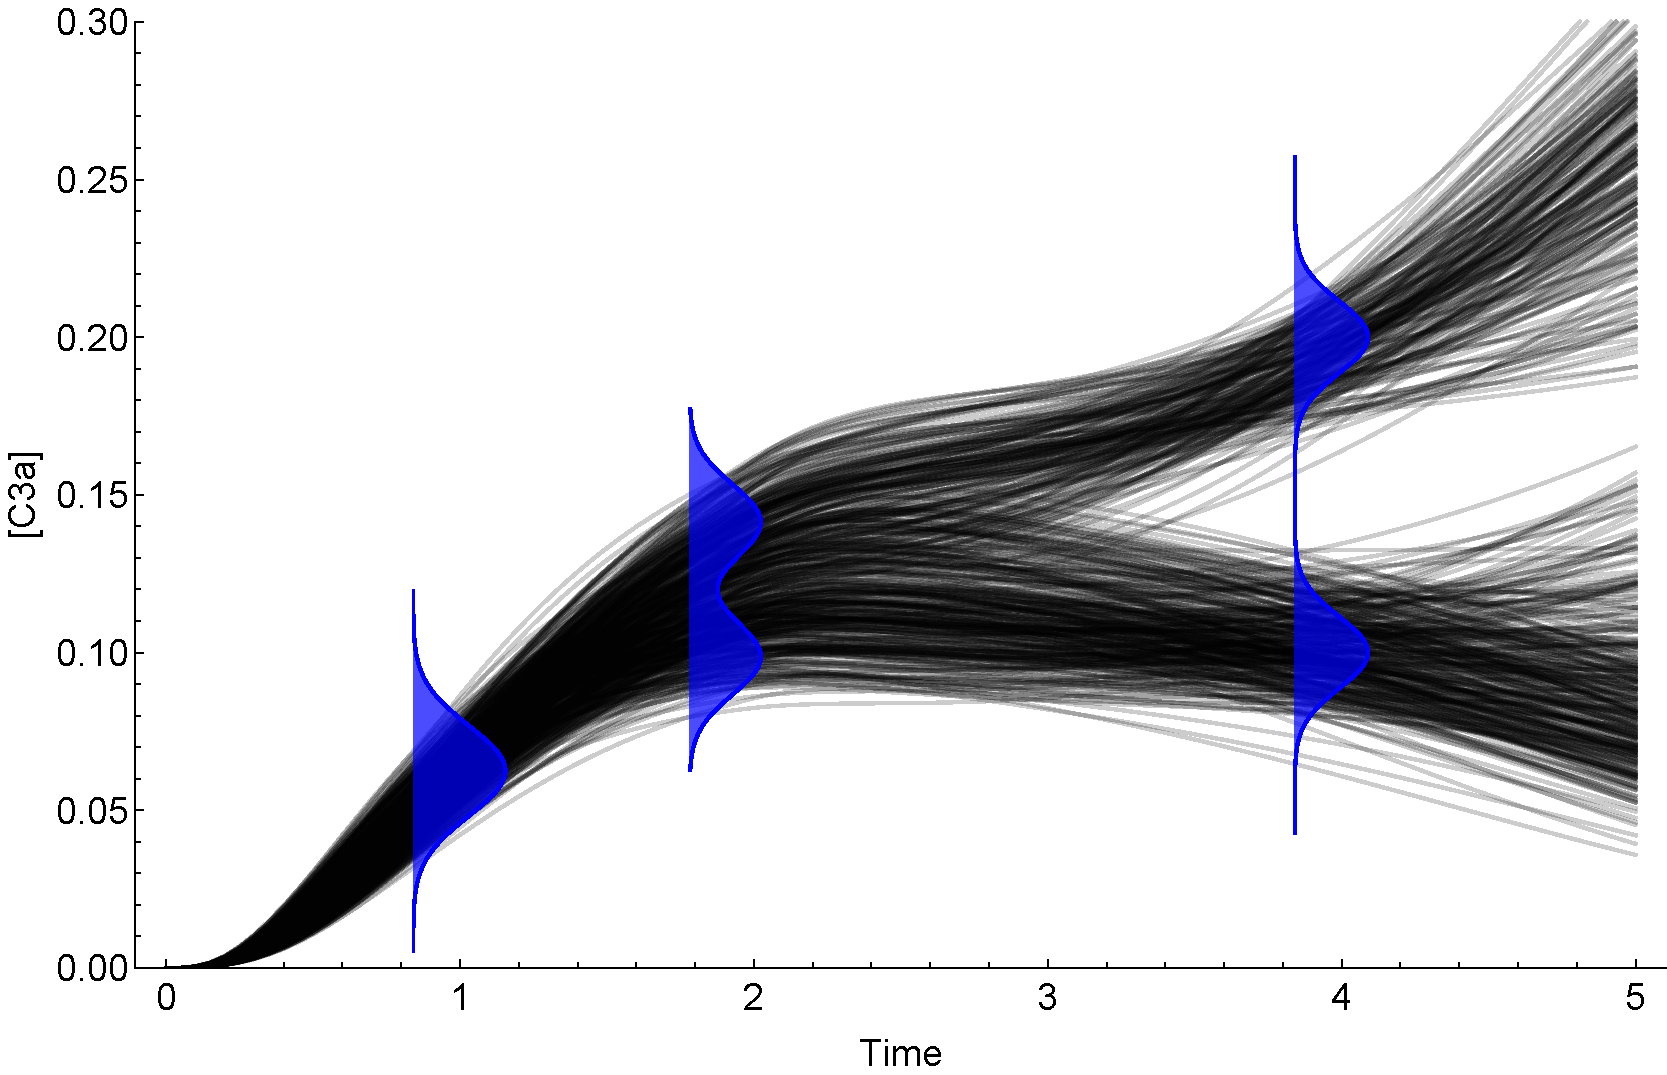
\includegraphics[width=0.8\textwidth]{../figures/tnf_samples_vs_distribution.pdf}}
	\caption{\textbf{The target output distribution (dashed plots with grey filling) and unique trajectories (black solid lines) obtained from the posterior parameter distribution.} In CMC, 10,000 independent samples were used in the ``ContourVolumeEstimator'' step and 5,000 MCMC samples across each of 4 Markov chains were used in the second step, with the first half of the chains discarded as ``warm-up'' \cite{lambert2018Student}.}
	\label{fig:tnf_samples_vs_distribution}
\end{figure}

\begin{table}[H]
\centering
%\scriptsize
\begin{adjustwidth}{0in}{0in}%
\begin{tabularx}{1.0\textwidth}{llclcc}
Model	& Target  & Parameter & Prior    & Prior  & Prior  \\
        & density &           & density  & $p_1$  & $p_2$  \\
\toprule
Growth  & 2D     & $R_T$       & uniform & $2.5 \times 10^5$ &  $8 \times 10^5$\\
factor  & normal & $k_1$       & uniform & 0.25 & 3.0\\
                && $k_{-1}$    & uniform & 2.0 & 20.0\\
                && $k_{deg}$   & uniform & 0.005 & 0.03\\
                && $k^*_{deg}$ & uniform & 0.1 & 0.5\\
\toprule
Growth  & 2D     & $R_T$ & normal & $5 \times 10^5$ &  $1 \times 10^5$\\
factor  & normal & $k_1$ & normal & 0.5 & 0.1\\
                && $k_{-1}$ & normal & 3.0 & 1.0\\
                && $k_{deg}$ & normal & 0.02 & 0.005\\
                && $k^*_{deg}$ & normal & 0.3 & 0.1\\
\toprule
Michaelis- & bimodal  & $k_f$ & uniform & 0.2 &  15\\
Menten     & normal   & $k_r$ & uniform & 0.2 & 2.0\\
&& $k_{cat}$ & uniform & 0.5 & 3.0\\
\toprule
Michaelis- & 4D    & $k_f$ & uniform & 0.2 &  15\\
Menten     & normal& $k_r$ & uniform & 0.2 & 2.0\\
&& $k_{cat}$ & uniform & 0.2 & 3.0\\
&& $E_0$ & uniform & 3.0 & 5.0\\
&& $S_0$ & uniform & 5.0 & 10.0\\
&& $C_0$ & uniform & 0.0 & 0.2\\
&& $P_0$ & uniform & 0.0 & 0.2\\
\toprule
TNF & bivariate & $a_1$ & uniform & 0.4 & 0.8\\
signalling & normal& $a_2$ & uniform & 0.1 & 0.7\\
&& $a_3$ & uniform & 0.3 & 0.7\\
&& $a_4$ & uniform & 0.1 & 0.3\\
&& $b_1$ & uniform & 0.5 & 0.7\\
&& $b_2$ & uniform & 0.4 & 0.6\\
&& $b_3$ & uniform & 0.4 & 0.6\\
&& $b_4$ & uniform & 0.2 & 0.4\\
&& $b_5$ & uniform & 0.2 & 0.4\\
\toprule
TNF  & bimodal  & $a_1$ & uniform & 0.5 & 0.7\\
signalling& normal & $a_2$ & uniform & 0.1 & 0.3\\
&& $a_3$ & uniform & 0.1 & 0.3\\
&& $a_4$ & uniform & 0.4 & 0.6\\
&& $b_1$ & uniform & 0.3 & 0.5\\
&& $b_2$ & uniform & 0.6 & 0.8\\
&& $b_3$ & uniform & 0.2 & 0.4\\
&& $b_4$ & uniform & 0.4 & 0.6\\
&& $b_5$ & uniform & 0.3 & 0.5\\
\end{tabularx}
\caption{\textbf{The priors used for each problem in \S\ref{sec:results}.}}
\label{tab:priors}
\end{adjustwidth}
\end{table}
